\documentclass[12pt,letterpaper]{report}

\usepackage[spanish]{babel}
\usepackage[utf8]{inputenc}
\usepackage{csquotes}
\usepackage[T1]{fontenc}
\usepackage{caption}
\usepackage{subcaption}
\captionsetup[figure]{justification=centering}
\usepackage[style=apa, backend=biber, language=spanish]{biblatex}
\addbibresource{referencias.bib}
\usepackage{graphicx}
\usepackage[table]{xcolor}
\definecolor{purplet}{RGB}{126, 103, 166}
\usepackage[hidelinks]{hyperref}
\usepackage{tikz}
\usetikzlibrary{arrows.meta,positioning,shapes.geometric,fit,calc}

\usepackage{geometry}
\geometry{
  left=3cm,
  right=2cm,
  top=2cm,
  bottom=2cm
}

\usepackage{setspace}
\usepackage{parskip}
\usepackage{ragged2e}
\usepackage{float}
\usepackage{array}
\usepackage{tabularx}
\usepackage{booktabs}

\usepackage{tocloft}
\setlength{\parindent}{0pt}

\addto\captionsspanish{
  \renewcommand{\contentsname}{ÍNDICE GENERAL}
  \renewcommand{\listfigurename}{ÍNDICE DE FIGURAS}
  \renewcommand{\listtablename}{ÍNDICE DE TABLAS}
}

\setlength{\cftbeforetoctitleskip}{0pt}
\setlength{\cftbeforeloftitleskip}{0pt}
\setlength{\cftbeforelottitleskip}{0pt}
\setlength{\cftaftertoctitleskip}{12pt}
\setlength{\cftafterloftitleskip}{12pt}
\setlength{\cftafterlottitleskip}{12pt}

\renewcommand{\cfttoctitlefont}{\fontsize{12}{14}\selectfont\bfseries}
\renewcommand{\cftloftitlefont}{\fontsize{12}{14}\selectfont\bfseries}
\renewcommand{\cftlottitlefont}{\fontsize{12}{14}\selectfont\bfseries}

\usepackage{titlesec}

\titleformat{\chapter}[block]
  {\fontsize{12}{14}\selectfont\bfseries\centering}
  {CAPÍTULO \Roman{chapter}.}
  {0.5em}
  {\MakeUppercase}
\titlespacing*{\chapter}{0pt}{6pt}{6pt}

\titleformat{\section}[block]
  {\fontsize{12}{14}\selectfont\bfseries}
  {\thesection}
  {0.5em}
  {}
\titlespacing*{\section}{0pt}{6pt}{6pt}

\titleformat{\subsection}[block]
  {\fontsize{11}{13}\selectfont\bfseries}
  {\thesubsection}
  {0.5em}
  {}
\titlespacing*{\subsection}{0pt}{6pt}{6pt}

\titleformat{\subsubsection}[block]
  {\fontsize{11}{13}\selectfont\normalfont}
  {\thesubsubsection}
  {0.5em}
  {}
\titlespacing*{\subsubsection}{0pt}{6pt}{6pt}

% \counterwithout{figure}{chapter}

\usepackage{fancyhdr}
\pagestyle{fancy}
\fancyhf{}
\fancyfoot[C]{\thepage}
\renewcommand{\headrulewidth}{0pt}

\AtBeginDocument{%
  \singlespacing
  \setlength{\parskip}{6pt}
  \justifying
}

\begin{document}

\begin{titlepage}
\centering
\vspace*{0cm}
\begin{minipage}[c]{0.18\textwidth}
  \centering
  
\includegraphics[width=0.8\textwidth]{assets/logo_left.png}
\end{minipage}%
\hfill
\begin{minipage}[c]{0.64\textwidth}
  \centering
  {\fontsize{12}{15}\selectfont\bfseries
  UNIVERSIDAD MAYOR DE SAN SIMÓN\\[4pt]
  FACULTAD DE CIENCIAS Y TECNOLOGÍA\\[4pt]
  CARRERA DE INGENIERÍA INFORMÁTICA}
\end{minipage}%
\hfill
\begin{minipage}[c]{0.18\textwidth}
  \centering
  
\includegraphics[width=0.9\textwidth]{assets/logo_right.png}
\end{minipage}

\vspace{3cm}

{\fontsize{16}{32}\selectfont\bfseries SISTEMA WEB PARA LA ADMINISTRACIÓN \\[0.4cm] DEL DESAFÍO BEBRAS EN BOLIVIA}\\[0.4cm]
\vspace{0.5cm}

{\large{Adscripción presentado para optar al Diploma Académico de Licenciatura en Ingeniería Informática}}\\[0.3cm]

\vspace{2cm}

\setstretch{1.6}
{\large
\textbf{Presentado por:}\\[6pt]
Castro Tejada Steven Lisandro\\
Velasquez Vela Marcos\\[8pt]
\textbf{Tutor:} Lic. Blanco Coca Leticia\\[8pt]
\textbf{Supervisor:} Lic. Costas Jauregui Vladimir Abel\\[8pt]

}

\vfill

{\large\bfseries COCHABAMBA -- BOLIVIA}\\[4pt]
{\normalsize Abril -- 2026}

\end{titlepage}

\begin{center}
{\fontsize{14}{16}\selectfont\bfseries DEDICATORIA}
\end{center}
\newpage
\begin{center}
{\fontsize{14}{16}\selectfont\bfseries AGRADECIMIENTOS}
\end{center}
\newpage

\clearpage
\tableofcontents
\clearpage
\listoffigures
\clearpage
\listoftables
\clearpage

\chapter{INTRODUCCIÓN}

En las últimas dos décadas, la informática ha dejado de ser un campo reservado exclusivamente a especialistas para convertirse en una competencia transversal con impacto en la vida cotidiana, la educación y el trabajo. Comprender cómo se representan los problemas, cómo se estructuran las soluciones y cómo se diseñan procesos ordenados para resolverlos constituye hoy una necesidad formativa cada vez más relevante, incluso para personas que no se dedicarán profesionalmente al desarrollo de software. En este contexto, el pensamiento computacional ha adquirido un papel central dentro de las discusiones educativas contemporáneas, al proponer una forma de razonamiento basada en la descomposición de problemas, el reconocimiento de patrones, la abstracción y el diseño de procedimientos paso a paso.

Sin embargo, la incorporación del pensamiento computacional en contextos escolares plantea un desafío importante: no basta con reconocer su valor teórico, sino que es necesario traducirlo en experiencias educativas accesibles, motivadoras y adecuadas a la edad de los estudiantes. En muchos casos, la enseñanza de conceptos vinculados a la informática se confunde con la enseñanza de programación o con el uso instrumental de herramientas digitales, lo que limita su alcance pedagógico. Frente a esta situación, han surgido iniciativas internacionales que buscan acercar los fundamentos de la informática a niños y jóvenes sin exigir conocimientos técnicos previos. Entre ellas, una de las más consolidadas es el Desafío Bebras.

El Desafío Bebras es una competencia internacional orientada a promover el pensamiento computacional mediante tareas breves que plantean problemas de lógica, representación, secuencias, estructuras, algoritmos y análisis de situaciones. Su rasgo más distintivo es que no exige saber programar para participar. En lugar de evaluar dominio de lenguajes o herramientas informáticas, propone ejercicios diseñados para que los estudiantes razonen sobre conceptos fundamentales de las ciencias de la computación a partir de situaciones cercanas, visuales o lúdicas. Gracias a este enfoque, Bebras se ha consolidado como una de las experiencias educativas más difundidas para introducir la informática en niveles escolares, mediante una red internacional en la que cada país organiza su propia edición nacional del desafío.

La relevancia de Bebras no se limita a su dimensión pedagógica. Su implementación práctica requiere una infraestructura tecnológica capaz de administrar procesos que van más allá de la simple publicación de ejercicios. Una edición nacional del desafío necesita gestionar participantes, categorías, tareas, pruebas y resultados de manera confiable. En consecuencia, la realización sostenida del concurso depende no solo de criterios educativos, sino también de una plataforma tecnológica que permita operarlo de manera ordenada, segura y escalable.

En distintos países, estas necesidades han dado lugar al desarrollo de plataformas propias, adaptadas a sus contextos organizativos, pedagógicos y técnicos. No existe un único sistema oficial compartido por todos los miembros de la red Bebras, sino una diversidad de implementaciones nacionales que responden a distintas prioridades: algunas se centran en la administración del concurso, otras en la práctica libre de tareas y otras en la comunicación institucional con docentes, familias y coordinadores. Esta diversidad responde al propio modelo de organización de Bebras, que opera mediante estructuras nacionales responsables de ejecutar el desafío en cada país. Por ello, el problema no consiste únicamente en disponer de tareas o materiales, sino en contar con una solución integral capaz de sostener la operación local del desafío.

En Bolivia, esta situación adquiere particular relevancia. A pesar del valor formativo del pensamiento computacional y del crecimiento internacional de Bebras, no se cuenta con una plataforma web propia que permita organizar de forma estable una edición nacional del desafío. Esta carencia resulta especialmente significativa en el contexto de la participación prevista de Bolivia en 2026, ya que la ausencia de infraestructura dificulta la inscripción de participantes, la administración de evaluaciones en línea, la gestión de contenido académico y la consolidación institucional de la iniciativa. Como resultado, la incorporación boliviana a este tipo de experiencias se ve condicionada por barreras operativas que no dependen del interés pedagógico del modelo, sino de la falta de un sistema adecuado para implementarlo en el contexto nacional.

A partir de este problema, el presente trabajo se orienta al desarrollo de la plataforma web del Desafío Bebras Bolivia. La propuesta no se restringe a la construcción de un sitio informativo, sino que plantea un sistema capaz de cubrir los procesos esenciales para la realización del concurso: difusión institucional, inscripción de usuarios, administración de exámenes, resolución de tareas y gestión de ejercicios. De este modo, el proyecto se sitúa en la intersección entre la informática educativa y el desarrollo de software.

Para una persona ajena al tema, es importante entender que este trabajo no busca simplemente digitalizar un examen, sino crear las condiciones técnicas para que una iniciativa educativa internacional pueda existir de forma sostenible en Bolivia. Eso implica comprender, por un lado, qué es el pensamiento computacional y por qué Bebras representa un modelo pertinente para promoverlo y, por otro, qué requerimientos debe cumplir una plataforma web para administrar un concurso educativo de este tipo. Bajo esa lógica, el documento avanza desde los fundamentos conceptuales del desafío hacia el análisis de plataformas de referencia y la definición de una solución tecnológica ajustada al contexto boliviano.

En consecuencia, el presente documento se organiza del siguiente modo. En el capítulo siguiente se desarrollan el marco conceptual y el estado del arte, abordando el pensamiento computacional, la organización internacional Bebras, los criterios para el diseño de tareas y los antecedentes relevantes a nivel internacional y regional. Posteriormente, se expone la metodología adoptada y el marco tecnológico que sustenta la propuesta, incluyendo la retroingeniería de plataformas de referencia y la justificación de las herramientas seleccionadas para la implementación del sistema. Con ello, el trabajo busca fundamentar de manera integral la necesidad y viabilidad de una plataforma web propia para el Desafío Bebras Bolivia.


\input{content/02_marco_conceptual.tex}

\chapter{METODOLOGÍA Y MARCO TECNOLÓGICO}

El presente capítulo describe el enfoque metodológico y las decisiones tecnológicas adoptadas para el desarrollo del sistema Bebras Bolivia. En primer lugar, se analizan plataformas nacionales de referencia con el propósito de identificar patrones de arquitectura, módulos funcionales y criterios de diseño reutilizables. Posteriormente, se examina la naturaleza de los sistemas de gestión de concursos en línea, distinguiéndolos de otras plataformas educativas y precisando los requisitos operativos que condicionan su implementación.

Finalmente, se presentan las herramientas y tecnologías seleccionadas para la construcción del sistema, justificando su elección en función de criterios de rendimiento, mantenibilidad, coherencia de pila y adecuación al contexto del proyecto. Esta exposición metodológica y tecnológica permite fundamentar la solución propuesta no solo desde el punto de vista conceptual, sino también desde su viabilidad práctica e implementación efectiva.

\section{ANÁLISIS COMPARATIVO DE PLATAFORMAS BEBRAS DE REFERENCIA}

Con el propósito de fundamentar las decisiones de diseño funcional, arquitectónico y de interfaz del sistema propuesto para Bebras Bolivia, se realizó un análisis comparativo sobre un conjunto de implementaciones nacionales del Desafío Bebras. Este análisis no se limitó a una descripción general de los sitios o repositorios disponibles, sino que buscó identificar de manera sistemática, a partir de la observación de su funcionamiento y de la información técnica pública disponible, los componentes, patrones de organización, módulos funcionales y estrategias de interacción más relevantes de cada plataforma revisada.

La selección de los casos de estudio respondió a criterios complementarios: disponibilidad de código fuente o información técnica pública, grado de madurez de la implementación, representatividad dentro del ecosistema Bebras y utilidad como referencia para el contexto boliviano. A partir de esta revisión, fue posible reconocer fortalezas particulares en cada plataforma y extraer de ellas los elementos más valiosos para la definición de la propuesta tecnológica del presente trabajo. En consecuencia, el análisis realizado no tuvo como finalidad replicar una solución existente, sino sintetizar buenas prácticas dispersas en distintas implementaciones nacionales para integrarlas en un sistema propio, coherente con los requerimientos de Bebras Bolivia.

\subsection{Plataforma de Francia --- Castor Informatique}

La implementación francesa, \emph{Castor Informatique}, mantenida por France-IOI, constituye una de las referencias más consolidadas dentro del ecosistema Bebras y dispone de código fuente accesible públicamente \parencite{bebrasfrancia}. El análisis de su estructura permitió identificar una separación clara entre módulos de concurso, maestros y preguntas, así como una estrategia orientada a optimizar la entrega de contenido mediante generación o compilación previa de materiales de prueba.

Desde la perspectiva de este análisis, el principal aporte de esta plataforma radica en su eficiencia para servir contenido y en la organización clara de sus componentes funcionales. Para Bebras Bolivia, esta referencia resultó especialmente útil en la definición de estrategias de entrega de contenido y en la inspiración de un esquema modular para separar áreas públicas, administrativas y de evaluación.

\subsection{Plataforma de Bélgica --- Rasbeb2}

La plataforma belga \emph{Rasbeb2}, disponible bajo licencia MIT \parencite{bebrasbelgica}, presenta una arquitectura orientada a la gestión integral del concurso. Su implementación en Java y su organización por módulos administrativos, tareas interactivas y documentación permitieron identificar una estructura robusta para el manejo de procesos internos del sistema.

El principal valor extraído de esta plataforma fue su diseño modular aplicado al flujo del concurso, particularmente en la separación entre inscripción, administración, ejecución y evaluación. Aunque no se adoptó su base tecnológica, su organización interna aportó criterios relevantes para estructurar el sistema Bebras Bolivia desde una lógica funcional más que desde una lógica de simple desarrollo web.

\subsection{Plataforma de Perú --- Bebras Perú}

La plataforma de Bebras Perú \parencite{bebrasperu} ofrece una referencia importante desde el punto de vista comunicacional e institucional. Su sitio prioriza la presentación pública de información para maestros, instituciones educativas y participantes, organizando con claridad niveles, recursos, orientaciones y mecanismos de inscripción.

A partir del análisis de esta plataforma, se identificó como fortaleza principal la claridad en la arquitectura de información orientada a usuarios no técnicos. Este aspecto fue considerado especialmente valioso para el diseño del sitio informativo de Bebras Bolivia, ya que evidencia la necesidad de estructurar el contenido de manera diferenciada para instituciones educativas, maestros, estudiantes y familias.

\subsection{Plataforma de Estados Unidos --- Bebras Computing Challenge}

La plataforma de \textcite{bebraseeuu} combina un entorno de práctica abierta con acceso a tareas de ediciones anteriores y un espacio de gestión dirigido a responsables institucionales. Su interfaz organiza de forma clara las categorías, el formato del concurso y los mecanismos de participación, al mismo tiempo que ofrece una experiencia de resolución de ejercicios bien definida.

Desde el análisis realizado, su principal aporte fue el modelo de interacción del módulo de ejercicios, especialmente en aspectos como la presentación del problema, la navegación entre tareas, la retroalimentación al usuario y la integración entre práctica y evaluación. Estos elementos sirvieron como referencia directa para definir la experiencia de uso esperada en el módulo de resolución de tareas de Bebras Bolivia.

\subsection{Síntesis de aportes extraídos del análisis comparativo}

El análisis comparativo de las plataformas revisadas permitió concluir que no existe una única implementación que resuelva de manera integral todos los requerimientos identificados para Bebras Bolivia. Sin embargo, cada una de las referencias estudiadas aporta fortalezas concretas que pueden ser integradas en una propuesta propia. En este sentido, el presente proyecto no se plantea como una réplica de ninguna plataforma existente, sino como una síntesis de buenas prácticas funcionales, arquitectónicas y de interfaz observadas en distintas implementaciones nacionales del ecosistema Bebras.

\begin{table}[H]
\centering
\caption[Elementos recuperados de plataformas Bebras de referencia]{Elementos recuperados mediante el análisis comparativo de plataformas Bebras de referencia y su aplicación en Bebras Bolivia}
\label{tab:retro_bebras}
\renewcommand{\arraystretch}{1.25}
\begin{tabular}{|p{3.5cm}|p{4.8cm}|p{6cm}|}
\hline
\textbf{Plataforma} & \textbf{Elemento rescatado} & \textbf{Aplicación} \\ \hline
Castor Informatique & Separación entre concurso, maestros y banco de preguntas; publicación eficiente de contenidos & Base para dividir el sistema en módulos administrativos, académicos y de evaluación, y para orientar la entrega optimizada de tareas y recursos \\ \hline
Rasbeb2 & Organización modular del flujo del concurso y soporte para tareas interactivas & Referencia para estructurar los procesos de inscripción, ejecución, corrección y administración del concurso dentro del CMS \\ \hline
Bebras Perú & Arquitectura de información clara para maestros, instituciones y postulantes & Base para diseñar el sitio informativo y ordenar la comunicación institucional según tipo de usuario \\ \hline
Bebras Computing Challenge & Presentación de tareas, práctica previa y navegación entre ejercicios & Referencia para definir la experiencia del participante en el módulo de resolución de tareas y práctica \\ \hline
\end{tabular}
\end{table}

\section{SISTEMAS DE GESTIÓN DE CONCURSOS EN LÍNEA}

Un sistema de gestión de concursos en línea es una plataforma web que administra de manera integral el ciclo de vida de una competencia: el registro de participantes e instituciones, la configuración y distribución de pruebas, la ejecución controlada de exámenes en sesiones con tiempo limitado, la evaluación automática de respuestas y la publicación de resultados. Este tipo de sistemas se articula en torno a tres funciones esenciales: la autenticación segura de los participantes, la gestión del banco de preguntas y el motor de evaluación automática. Estos tres componentes están presentes en todas las implementaciones nacionales de Bebras analizadas y definen igualmente los módulos centrales del sistema desarrollado en este proyecto.

A diferencia de un sistema de gestión de aprendizaje (\textit{Learning Management System}, LMS) de propósito general, un sistema de gestión de concursos educativos debe garantizar condiciones equivalentes para todos los participantes durante la ejecución de la prueba: disponibilidad simultánea para múltiples sesiones concurrentes, control estricto del tiempo por participante y registro confiable de respuestas ante posibles interrupciones de conectividad. Estos requisitos condicionan directamente las decisiones de arquitectura del sistema propuesto.

La distinción funcional entre un sistema de gestión de concursos y un LMS se ilustra en la Figura~\ref{fig:cms_vs_lms}.

\begin{figure}[htbp]
    \centering
    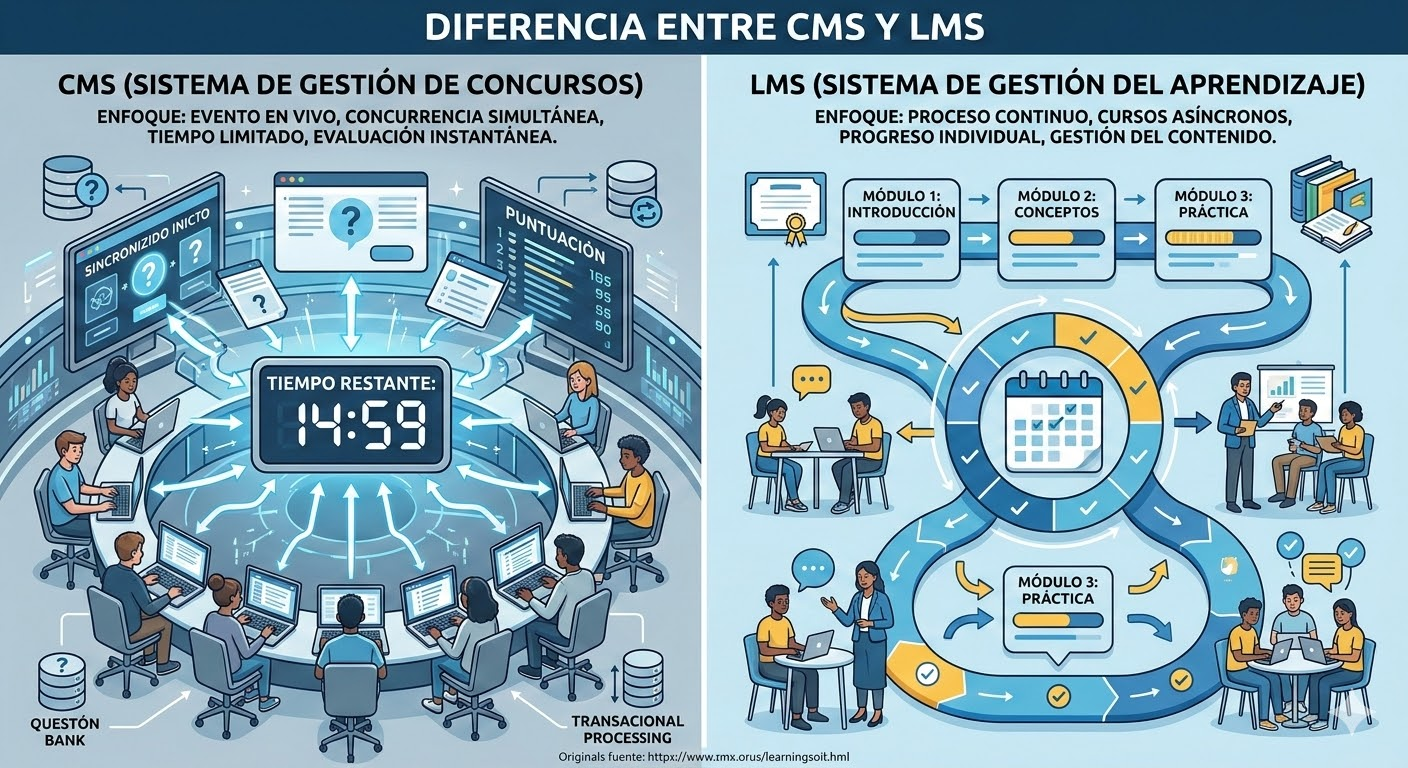
\includegraphics[width=0.70\textwidth]{assets/cms_vs_lms.jpg}
    \caption[Comparación entre CMS y LMS]{Comparación conceptual entre un \textit{Contest Management System} y un \textit{Learning Management System}}
    \label{fig:cms_vs_lms}
\end{figure}

\section{METODOLOGÍA DE ANÁLISIS Y DISEÑO}

La metodología adoptada en este trabajo combina revisión documental, análisis comparativo de plataformas de referencia y definición de una arquitectura ajustada a los requisitos funcionales y no funcionales del proyecto. En una primera etapa, se realizó una revisión de literatura especializada sobre pensamiento computacional, el modelo Bebras y la construcción de tareas educativas de informática. En una segunda etapa, se analizaron distintas plataformas nacionales de Bebras con el fin de identificar módulos recurrentes, patrones de interacción y decisiones arquitectónicas relevantes.

Sobre la base de este análisis, se procedió a definir los módulos que conforman la propuesta tecnológica para Bebras Bolivia: gestión de contenido y sitio informativo, gestión de competencias, registro de participantes y evaluación digital e imprimible. Finalmente, se seleccionó una pila tecnológica coherente con los requerimientos de rendimiento, mantenibilidad y escalabilidad identificados durante el proceso.

\subsection{Extreme Programming (XP)}

El desarrollo del presente proyecto adoptó \textit{Extreme Programming} (XP) como metodología ágil de referencia. XP fue propuesto por \textcite{beck2004} como un enfoque orientado a equipos pequeños que trabajan sobre requisitos cambiantes, priorizando la entrega continua de software funcional y la incorporación sistemática de retroalimentación. Estas características lo hacen especialmente adecuado para un proyecto de grado en el que el desarrollo avanza de forma incremental, con revisiones periódicas por parte del supervisor y ajustes continuos al alcance y al diseño del sistema.

La elección de XP como metodología de referencia se fundamenta en una comparación con otras alternativas ampliamente utilizadas. Scrum, aunque popular en equipos de desarrollo profesional, presupone roles diferenciados \textit{Product Owner}, \textit{Scrum Master} y equipo de desarrollo y una estructura de ceremonias formales que no se corresponden con el equipo reducido de dos desarrolladores que conforma este proyecto \parencite{schwaber2020}. Kanban, por su parte, ofrece flexibilidad en la gestión del flujo de trabajo, pero carece de los mecanismos de planificación por valores y retroalimentación continua que XP incorpora de manera explícita \parencite{anderson2010}. En contraste, XP está diseñado para contextos donde el equipo es reducido, los requisitos evolucionan durante el desarrollo y la calidad del software es una prioridad sostenida a lo largo de todo el proceso.

XP se articula en torno a cinco valores fundamentales que orientan las decisiones de diseño y desarrollo \parencite{beck2004}. La \textit{comunicación} se manifiesta en este proyecto a través del diálogo continuo con el supervisor, que permite alinear expectativas y corregir el rumbo en cada ciclo de avance. La \textit{simplicidad} guía las decisiones de arquitectura y diseño de módulos, priorizando soluciones directas y mantenibles sobre implementaciones sobredimensionadas. La \textit{retroalimentación} opera como mecanismo central de validación: cada entrega parcial es revisada y genera insumos concretos para la iteración siguiente. La \textit{valentía} se refleja en la disposición a refactorizar o rediseñar componentes cuando el análisis lo justifica, sin preservar decisiones técnicas por inercia. Finalmente, el \textit{respeto} se traduce en el cuidado por producir un sistema coherente, bien documentado y sostenible más allá del alcance inmediato del proyecto.

De las prácticas que XP propone, este proyecto incorpora de manera explícita el desarrollo iterativo e incremental, la integración continua de retroalimentación como insumo de corrección, la validación sostenida de decisiones de diseño y arquitectura y la programación en pareja, práctica que resulta especialmente adecuada para un equipo de dos desarrolladores. No se adoptaron, en cambio, prácticas pensadas para equipos numerosos, como la propiedad colectiva del código a gran escala, dado que el proyecto es desarrollado por un equipo de dos personas con responsabilidades claramente delimitadas. Esta selección de prácticas de XP es consistente con lo señalado por \textcite{shore2021}, quienes reconocen que los equipos pueden adoptar un subconjunto coherente de prácticas XP sin comprometer los principios fundamentales de la metodología.

Siguiendo el principio de iteraciones cortas de duración fija propio de XP, el desarrollo se organizó mediante \textit{timeboxing}. En XP, las iteraciones suelen mantenerse dentro de rangos breves, comúnmente entre una y tres semanas, con el propósito de entregar incrementos verificables y recibir retroalimentación frecuente. Para el presente proyecto se adoptaron iteraciones de tres semanas, debido a que el desarrollo se realizó en paralelo con actividades de análisis, documentación, validación con el supervisor y refinamiento funcional del producto.

Dado que los módulos del sistema presentan distinta extensión y complejidad, no existe una correspondencia directa entre un módulo y una única iteración. En lugar de extender la duración de una iteración para acomodar un módulo de mayor tamaño, cada módulo se desarrolla a lo largo del número de iteraciones que requiera, manteniendo invariable la caja de tiempo de tres semanas.

\subsection{Diseño centrado en el usuario e interacción persona computadora}

Complementariamente a XP, el desarrollo del sistema incorporó principios de diseño centrado en el usuario (\textit{User-Centered Design}, UCD), definidos en la norma \textcite{iso9241210}. Este enfoque establece que las decisiones de diseño deben fundamentarse en el conocimiento de los usuarios, sus tareas y su contexto de uso, con el propósito de producir sistemas que sean utilizables, accesibles y adecuados a las necesidades reales de quienes los emplean.

La pertinencia de este enfoque en el presente proyecto se deriva de la diversidad de perfiles de usuario que interactúan con el sistema. La arquitectura funcional contempla tres actores principales: el \textbf{administrador u organizador}, responsable de la configuración global del concurso y de la administración del contenido; el \textbf{maestro}, encargado de articular la participación de su unidad educativa o grupo de estudiantes; y el \textbf{estudiante}, cuya interacción se concentra en el acceso y resolución de la prueba. Cada actor presenta competencias digitales, objetivos y contextos de uso diferentes, por lo que las decisiones de interfaz no pueden abordarse de manera uniforme. Las definiciones de navegación, estructura de información y presentación de contenido se orientaron en función de los requisitos específicos de cada rol, tomando como referencia los principios de usabilidad descritos por \textcite{norman2013}.

El módulo de resolución de tareas merece una atención particular desde la perspectiva de la interacción persona computadora (\textit{Human-Computer Interaction}, HCI). Al tratarse del componente con el que interactúan directamente los estudiantes, el grupo de usuarios con menor experiencia digital y mayor heterogeneidad etaria dentro del sistema, su diseño debe atender criterios de usabilidad, claridad visual y accesibilidad de manera rigurosa. \textcite{preece2015} señalan que el diseño de interfaces para usuarios con perfiles cognitivos y etarios diversos exige una atención especial a la carga cognitiva, la consistencia visual y la retroalimentación inmediata ante las acciones del usuario. En este contexto, aspectos como el contraste visual, la legibilidad tipográfica, la navegación entre tareas y la presentación del tiempo disponible no son decisiones estéticas, sino funcionales: condicionan directamente la capacidad del estudiante para concentrarse en la resolución del problema sin ser obstaculizado por la interfaz misma.

Adicionalmente, el sistema debe considerar criterios de accesibilidad web definidos por las \textit{Web Content Accessibility Guidelines} (WCAG) \parencite{w3c2023}, que establecen estándares internacionales para garantizar que el contenido digital sea perceptible, operable, comprensible y robusto para usuarios con distintas capacidades. Dado que el concurso está dirigido a estudiantes de nivel primario y secundario en un contexto educativo diverso, la accesibilidad no es un complemento opcional sino un requisito de equidad: un sistema que no puede ser utilizado eficazmente por todos los participantes compromete la validez misma del concurso.

\section{MARCO TECNOLÓGICO}

El objetivo técnico central de este proyecto es el desarrollo de un sistema capaz de administrar de extremo a extremo el ciclo de vida del Desafío Bebras Bolivia: inscripción de instituciones y participantes, configuración y distribución de exámenes, ejecución controlada de pruebas en línea, registro automático de respuestas y consulta de resultados. A este sistema se suma un sitio informativo con capacidades propias de gestión de contenido, orientado a la comunicación institucional del desafío. La selección de tecnologías responde a criterios de rendimiento, coherencia de pila y mantenibilidad a largo plazo, considerando que ambos módulos deben operar de manera integrada sobre el mismo entorno de ejecución.

\subsection{Astro}

Astro fue seleccionado para el sitio informativo por su enfoque en rendimiento y generación de contenido estático. \textcite{astro} destaca su modelo \textit{server-first} y la \emph{Islands Architecture}, que hidrata solo los componentes interactivos y reduce JavaScript en cliente. Además, su integración con \textit{Content Collections} permite administrar contenido institucional de forma tipada y mantenible, en coherencia con la pila basada en Bun.

\subsection{Bun}

Bun se utiliza como entorno de ejecución unificado para JavaScript y TypeScript en el proyecto. \textcite{bun} lo describe como una alternativa de alto rendimiento que integra \textit{runtime}, gestor de paquetes y herramientas de desarrollo en una sola tecnología. Esta unificación simplifica la operación del sistema y reduce tiempos de ejecución y despliegue frente a cadenas de herramientas separadas.

\subsection{Express}

Express se eligió para la capa API del sistema por su arquitectura modular basada en \textit{middleware}. \textcite{express} resalta su flexibilidad para estructurar rutas, validaciones y control de errores sin imponer una arquitectura rígida. Esto ofrece una base adecuada para implementar flujos como autenticación, gestión de sesiones de examen y registro de respuestas dentro de un sistema de este tipo.

\subsection{Prisma ORM}

Prisma ORM se adoptó para el acceso a datos por su tipado estático en TypeScript y su manejo controlado de migraciones. \textcite{prisma} identifica como componentes centrales Prisma Client, Prisma Migrate y Prisma Studio. En este proyecto, \texttt{schema.prisma} funciona como fuente única de verdad del modelo, lo que mejora la consistencia del esquema y reduce errores de consulta en la integración con MariaDB.

\subsection{MariaDB}

MariaDB fue seleccionado como motor relacional del sistema por su madurez, licencia libre y compatibilidad con MySQL. De acuerdo con \textcite{mariadb}, mantiene compatibilidad de interfaces y bibliotecas, incorporando mejoras para entornos productivos. Su compatibilidad con Prisma ORM, mediante el conector de MySQL, lo convierte en una base sólida para la persistencia de datos del sistema.

La selección de las tecnologías descritas no respondió únicamente a criterios funcionales aislados, sino a una evaluación conjunta de sostenibilidad técnica, consumo de recursos, capacidad de escalamiento y afinidad con la experiencia previa del equipo de desarrollo. En este sentido, se priorizaron herramientas consolidadas, activamente mantenidas y adecuadas para una infraestructura moderada, evitando depender de soluciones excesivamente recientes o inciertas en su continuidad. La Tabla~\ref{tab:criterios_tecnologias} sintetiza estos criterios de selección.

    \begin{table}[H]
    \centering
    \caption[Criterios de selección de tecnologías]{Criterios que fundamentan la selección de las tecnologías del proyecto}
    \label{tab:criterios_tecnologias}
    \renewcommand{\arraystretch}{1.2}
    \begin{tabular}{|p{2.8cm}|p{4.2cm}|p{6.5cm}|}
    \hline
    \textbf{Tecnología} & \textbf{Criterio principal} & \textbf{Justificación} \\ \hline
    Astro & Eficiencia y optimización en frontend & El sitio informativo no requiere reactividad compleja; minimizar JavaScript en cliente reduce tiempos de carga en conexiones lentas, condición frecuente en el contexto boliviano. 
    \\ \hline
    Bun & Rendimiento y entorno unificado & Eliminar la separación entre runtime y gestor de paquetes reduce la superficie de configuración en un proyecto mantenido por un equipo pequeño. 
    \\ \hline
    Express & Estabilidad y curva de aprendizaje baja & El equipo cuenta con experiencia previa en Express, lo que reduce el riesgo técnico en flujos críticos como la gestión de sesiones de examen. 
    \\ \hline
    Prisma ORM & Mantenibilidad del modelo de datos & El esquema del concurso evolucionará durante el desarrollo; un ORM con migraciones tipadas reduce el riesgo de inconsistencias entre el modelo y la base de datos. 
    \\ \hline
    MariaDB & Madurez y bajo costo operativo & La infraestructura disponible para el proyecto es moderada; MariaDB opera eficientemente en ese contexto sin requerir configuración compleja.
    \\ \hline
    \end{tabular}
    \end{table}


\chapter{ARQUITECTURA E INTERACCIÓN DEL SISTEMA}

El presente capítulo describe la arquitectura funcional de la plataforma Bebras Bolivia y la forma en que sus módulos se relacionan para cubrir el ciclo operativo del desafío. La finalidad de esta sección es proporcionar una visión integral del sistema antes de abordar el desarrollo específico de cada módulo. Por ello, se identifican los actores principales, los módulos funcionales, los flujos de información y la secuencia general de operación del concurso.

La plataforma se concibe como un sistema modular. Cada módulo cumple un objetivo propio, pero no opera de manera aislada: el sitio informativo comunica el desafío, el módulo de inscripción registra participantes, el gestor de tareas y competencias organiza los contenidos de evaluación, y el módulo de evaluación ejecuta la participación y procesa resultados. Esta separación facilita el desarrollo incremental, permite distribuir responsabilidades y reduce la dependencia entre componentes.

\section{VISIÓN GENERAL DEL SISTEMA}

Bebras Bolivia se estructura como una plataforma web orientada a la gestión integral del Desafío Bebras en el contexto nacional. El sistema contempla desde la publicación de información institucional hasta la ejecución de la competencia, incorporando procesos de inscripción, administración de tareas, configuración de competencias y evaluación de respuestas.

La Figura~\ref{fig:vision_general_modulos} presenta una visión general de los cuatro módulos principales del sistema y su relación funcional.

\begin{figure}[H]
    \centering
    \fbox{\parbox{0.88\textwidth}{\centering
    \vspace{0.4cm}
    Diagrama general de módulos: CMS y sitio informativo, inscripción, gestor de tareas y competencias, evaluación.\\
    \vspace{0.4cm}
    }}
    \caption[Visión general de módulos]{Visión general de los módulos de la plataforma Bebras Bolivia - Elaboración propia}
    \label{fig:vision_general_modulos}
\end{figure}

\section{ESTRUCTURA FUNCIONAL DE LA PLATAFORMA}

\subsection{Actores del sistema}

Los actores del sistema representan los perfiles que interactúan con la plataforma según sus responsabilidades dentro del desafío. La Tabla~\ref{tab:actores_sistema} resume los actores identificados y el objetivo principal de cada uno.

\begin{table}[H]
\centering
\renewcommand{\arraystretch}{1.25}
\begin{tabular}{|p{4cm}|p{5.5cm}|p{5.5cm}|}
\hline
\textbf{Actor} & \textbf{Objetivo dentro del sistema} & \textbf{Módulos relacionados} \\ \hline
Visitante del sitio & Consultar información pública sobre el desafío, categorías, participación, preguntas frecuentes y canales de contacto & CMS y sitio informativo \\ \hline
Administrador del sitio & Mantener actualizado el contenido público, las publicaciones informativas, respaldos y publicación del sitio & CMS y sitio informativo \\ \hline
Coordinador institucional & Registrar la institución educativa y organizar la participación de estudiantes & Inscripción, evaluación \\ \hline
Docente & Orientar a los estudiantes, consultar información operativa y acompañar la participación & Sitio informativo, inscripción, evaluación \\ \hline
Estudiante & Participar en el desafío y resolver las tareas asignadas & Evaluación \\ \hline
Administrador de competencias & Registrar tareas, configurar competencias y definir parámetros de participación & Gestor de tareas y competencias, evaluación \\ \hline
\end{tabular}
\caption[Actores del sistema]{Actores principales de la plataforma Bebras Bolivia}
\label{tab:actores_sistema}
\end{table}

\subsection{Módulos principales de la plataforma}

La plataforma está compuesta por cuatro módulos principales. Cada módulo tiene una responsabilidad delimitada y produce información que puede ser consumida por otros módulos. La Tabla~\ref{tab:modulos_plataforma} presenta el objetivo, entrada y salida principal de cada módulo.

\begin{table}[H]
\centering
\renewcommand{\arraystretch}{1.25}
\begin{tabular}{|p{3.6cm}|p{4.6cm}|p{3.6cm}|p{3.6cm}|}
\hline
\textbf{Módulo} & \textbf{Objetivo} & \textbf{Entrada principal} & \textbf{Salida principal} \\ \hline
CMS y sitio informativo & Publicar y administrar información institucional del desafío & Contenido institucional, noticias, imágenes y configuración editorial & Sitio público actualizado \\ \hline
Inscripción & Registrar instituciones, docentes y estudiantes participantes & Datos de institución, coordinador y participantes & Listas de participantes habilitados \\ \hline
Gestor de tareas y competencias & Registrar tareas, organizar contenidos y configurar competencias & Tareas, categorías, niveles, fechas y parámetros de competencia & Competencias configuradas para evaluación \\ \hline
Evaluación & Ejecutar la participación, registrar respuestas y permitir el procesamiento de resultados & Participantes registrados y competencias configuradas & Respuestas, puntajes y resultados \\ \hline
\end{tabular}
\caption[Módulos principales de la plataforma]{Módulos funcionales de la plataforma Bebras Bolivia}
\label{tab:modulos_plataforma}
\end{table}

\section{INTERACCIÓN GENERAL DEL SISTEMA}

\subsection{Relación entre actores y módulos}

La interacción entre actores y módulos se define por el objetivo que cada actor cumple dentro del desafío. El visitante consulta información pública; el administrador del sitio mantiene actualizado el contenido; el coordinador institucional registra participantes; el administrador de competencias configura tareas y evaluaciones; y el estudiante participa en la competencia.

La Figura~\ref{fig:actores_modulos} muestra la relación conceptual entre los actores y los módulos principales.

\begin{figure}[H]
    \centering
    \fbox{\parbox{0.88\textwidth}{\centering
    \vspace{0.4cm}
    Diagrama actor-módulo: visitante y administrador del sitio con CMS; coordinador con inscripción; administrador de competencias con gestor de tareas; estudiante con evaluación.\\
    \vspace{0.4cm}
    }}
    \caption[Relación entre actores y módulos]{Relación entre actores y módulos funcionales de Bebras Bolivia - Elaboración propia}
    \label{fig:actores_modulos}
\end{figure}

\subsection{Articulación funcional de los módulos}

La arquitectura funcional del sistema se basa en una relación progresiva entre módulos. El CMS cumple una función comunicacional y editorial; el módulo de inscripción transforma el interés de participación en registros estructurados; el gestor de tareas prepara el contenido evaluativo; y el módulo de evaluación ejecuta la competencia usando los datos generados por inscripción y configuración de competencias.

La Figura~\ref{fig:interaccion_modulos} representa la articulación funcional entre módulos.

\begin{figure}[H]
    \centering
    \fbox{\parbox{0.88\textwidth}{\centering
    \vspace{0.4cm}
    Flujo de interacción: CMS informa; inscripción registra participantes; gestor configura tareas y competencias; evaluación consume participantes y competencias para generar resultados.\\
    \vspace{0.4cm}
    }}
    \caption[Interacción funcional entre módulos]{Interacción funcional entre los módulos de la plataforma - Elaboración propia}
    \label{fig:interaccion_modulos}
\end{figure}

\section{FLUJO OPERATIVO DEL DESAFÍO}

\subsection{Proceso general de funcionamiento}

El proceso operativo del desafío inicia con la publicación de información oficial en el sitio público. A partir de esa información, docentes, coordinadores y estudiantes conocen el objetivo del desafío, las categorías, las condiciones de participación y los canales de contacto. Posteriormente, el proceso continúa con la inscripción de instituciones y participantes, la preparación de tareas, la configuración de competencias, la ejecución de la evaluación y la generación de resultados.

\subsection{Secuencia operativa del concurso}

La secuencia funcional del concurso puede organizarse en siete etapas principales. La Tabla~\ref{tab:flujo_operativo} resume cada etapa y el módulo responsable.

\begin{table}[H]
\centering
\renewcommand{\arraystretch}{1.25}
\begin{tabular}{|p{1.5cm}|p{5cm}|p{5cm}|p{3.5cm}|}
\hline
\textbf{Nro.} & \textbf{Etapa} & \textbf{Descripción} & \textbf{Módulo principal} \\ \hline
1 & Publicación de información & Se comunica el desafío, categorías, instrucciones y canales de contacto & CMS y sitio informativo \\ \hline
2 & Registro de participación & Se registran instituciones, docentes y estudiantes & Inscripción \\ \hline
3 & Preparación de tareas & Se registran y validan tareas de pensamiento computacional & Gestor de tareas \\ \hline
4 & Configuración de competencia & Se definen fechas, duración, niveles y tareas asociadas & Gestor de competencias \\ \hline
5 & Ejecución de la evaluación & Los estudiantes resuelven tareas dentro del tiempo definido & Evaluación \\ \hline
6 & Registro de respuestas & El sistema almacena las respuestas generadas durante la participación & Evaluación \\ \hline
7 & Procesamiento de resultados & Se calculan puntajes, rankings o reportes según la configuración & Evaluación \\ \hline
\end{tabular}
\caption[Flujo operativo del desafío]{Secuencia operativa general del Desafío Bebras Bolivia}
\label{tab:flujo_operativo}
\end{table}

La Figura~\ref{fig:flujo_operativo} sintetiza visualmente el flujo operativo del desafío.

\begin{figure}[H]
    \centering
    \fbox{\parbox{0.88\textwidth}{\centering
    \vspace{0.4cm}
    Diagrama secuencial: publicación de información, inscripción, preparación de tareas, configuración de competencia, evaluación, respuestas y resultados.\\
    \vspace{0.4cm}
    }}
    \caption[Flujo operativo del desafío]{Flujo operativo general del Desafío Bebras Bolivia - Elaboración propia}
    \label{fig:flujo_operativo}
\end{figure}

\section{REPRESENTACIÓN GENERAL DEL SISTEMA}

\subsection{Mapa de interacción del sistema}

El mapa de interacción permite entender la plataforma como un conjunto de módulos coordinados. La separación modular evita que un único componente concentre todas las responsabilidades y permite que cada parte del sistema pueda evolucionar de forma controlada. En este sentido, el CMS no depende directamente de la evaluación, pero cumple una función inicial importante al comunicar el desafío y mantener actualizada la información pública.

\subsection{Diagrama general de módulos y procesos}

La Figura~\ref{fig:mapa_general_sistema} consolida los procesos y módulos principales en una representación única.

\begin{figure}[H]
    \centering
    \fbox{\parbox{0.88\textwidth}{\centering
    \vspace{0.4cm}
    Mapa general del sistema: actores, módulos, datos principales y flujo operativo del concurso.\\
    \vspace{0.4cm}
    }}
    \caption[Mapa general del sistema]{Mapa general de interacción del sistema Bebras Bolivia - Elaboración propia}
    \label{fig:mapa_general_sistema}
\end{figure}

En síntesis, la arquitectura propuesta permite organizar el sistema en componentes funcionales coherentes con el ciclo de vida del desafío. Esta visión modular sirve como base para documentar, en los capítulos siguientes, el desarrollo particular de cada módulo y su aporte al funcionamiento general de la plataforma.


\chapter{MÓDULO DE GESTIÓN DE CONTENIDO Y SITIO INFORMATIVO}

El presente capítulo describe el desarrollo del módulo de gestión de contenido y sitio informativo de Bebras Bolivia. Este módulo cumple una doble función: por una parte, presenta información pública sobre el desafío a estudiantes, docentes, coordinadores e instituciones interesadas; por otra, proporciona un panel de administración para mantener actualizado el contenido, administrar publicaciones informativas, revisar cambios, generar respaldos y publicar el sitio.

El desarrollo se organizó mediante iteraciones XP de tres semanas. La Iteración 0 se destinó a la preparación funcional y técnica del módulo; la Iteración 1 concentró la implementación del sitio informativo, el acceso al panel y la edición de páginas; y la Iteración 2 consolidó la gestión editorial, respaldos, vista previa y publicación del contenido.

\section{PLANIFICACIÓN DEL MÓDULO}

\subsection{Objetivo del módulo}

El objetivo del módulo es permitir la comunicación pública del Desafío Bebras Bolivia y facilitar la administración del contenido del sitio sin modificar directamente el código fuente. De esta manera, el sistema permite mantener actualizada la información institucional, las páginas informativas, las publicaciones y los recursos visuales asociados al desafío.

\subsection{Historias de usuario seleccionadas}

La Tabla~\ref{tab:historias_cms} presenta las historias de usuario consideradas para el desarrollo del módulo. Las tareas derivadas de estas historias fueron registradas como elementos relacionados en el tablero de proyecto, pero no se desarrollan como historias independientes dentro del documento.

\begin{table}[H]
\centering
\renewcommand{\arraystretch}{1.25}
\begin{tabular}{|p{2cm}|p{7cm}|p{3cm}|p{1.5cm}|p{1.5cm}|}
\hline
\textbf{ID} & \textbf{Historia} & \textbf{Usuario} & \textbf{Prioridad} & \textbf{Esf.} \\ \hline
CMS-00 & Preparar la base funcional del módulo & Equipo de desarrollo & 1 & 5 \\ \hline
CMS-01 & Presentar información pública del Desafío Bebras Bolivia & Visitante del sitio & 1 & 13 \\ \hline
CMS-02 & Controlar el acceso al panel de administración & Administrador del sitio & 1 & 5 \\ \hline
CMS-03 & Editar contenido de páginas informativas & Administrador del sitio & 1 & 13 \\ \hline
CMS-04 & Previsualizar cambios del sitio antes de publicarlos & Administrador del sitio & 1 & 8 \\ \hline
CMS-05 & Crear publicaciones informativas & Administrador del sitio & 1 & 5 \\ \hline
CMS-06 & Editar publicaciones informativas & Administrador del sitio & 1 & 8 \\ \hline
CMS-07 & Manejar imágenes para publicaciones informativas & Administrador del sitio & 2 & 5 \\ \hline
CMS-08 & Previsualizar publicaciones antes de guardarlas & Administrador del sitio & 1 & 5 \\ \hline
CMS-09 & Crear respaldos del contenido & Administrador del sitio & 1 & 5 \\ \hline
CMS-10 & Restaurar contenido desde un respaldo & Administrador del sitio & 1 & 8 \\ \hline
CMS-11 & Transferir respaldos del contenido & Administrador del sitio & 2 & 5 \\ \hline
CMS-12 & Publicar cambios del sitio informativo & Administrador del sitio & 1 & 8 \\ \hline
CMS-13 & Programar publicación del sitio informativo & Administrador del sitio & 2 & 5 \\ \hline
\end{tabular}
\caption[Historias de usuario del módulo CMS]{Historias de usuario seleccionadas para el módulo de gestión de contenido y sitio informativo}
\label{tab:historias_cms}
\end{table}

\subsection{Distribución por iteraciones}

La Tabla~\ref{tab:iteraciones_cms} muestra la distribución de las historias por iteración.

\begin{table}[H]
\centering
\renewcommand{\arraystretch}{1.25}
\begin{tabular}{|p{3cm}|p{9cm}|p{3cm}|}
\hline
\textbf{Iteración} & \textbf{Alcance principal} & \textbf{Historias} \\ \hline
Iteración 0 & Preparación funcional, tecnológica y estructural del módulo & CMS-00 \\ \hline
Iteración 1 & Sitio informativo, acceso administrativo, edición de contenido y vista previa del sitio & CMS-01, CMS-02, CMS-03, CMS-04 \\ \hline
Iteración 2 & Publicaciones informativas, imágenes, respaldos, restauración, transferencia y publicación & CMS-05 a CMS-13 \\ \hline
\end{tabular}
\caption[Distribución de historias por iteración]{Distribución de historias de usuario del módulo CMS por iteración}
\label{tab:iteraciones_cms}
\end{table}

\section{ITERACIÓN 0: PREPARACIÓN DEL MÓDULO}

\subsection{Planificación de la iteración}

La Iteración 0 se orientó a preparar la base del módulo. En esta etapa se definió el alcance del sitio informativo, se organizaron las páginas públicas, se seleccionó la pila tecnológica y se preparó la estructura inicial del repositorio. Esta iteración permitió establecer una base funcional sobre la cual se desarrollaron las historias de usuario de las siguientes iteraciones.

\subsection{Actividades principales}

\begin{table}[H]
\centering
\renewcommand{\arraystretch}{1.25}
\begin{tabular}{|p{3cm}|p{10cm}|p{2.5cm}|}
\hline
\textbf{ID} & \textbf{Actividad} & \textbf{Resultado} \\ \hline
CMS-00-01 & Definir el alcance del módulo de gestión de contenido y sitio informativo & Completado \\ \hline
CMS-00-02 & Seleccionar tecnologías para el sitio y el panel de administración & Completado \\ \hline
CMS-00-03 & Configurar la estructura inicial del repositorio & Completado \\ \hline
CMS-00-04 & Organizar páginas, datos editables y recursos visuales iniciales & Completado \\ \hline
\end{tabular}
\caption[Actividades de preparación del módulo]{Actividades realizadas durante la Iteración 0}
\label{tab:actividades_iteracion_0}
\end{table}

\subsection{Pruebas}

\subsubsection{Pruebas funcionales}

\subsubsection{Pruebas de configuración}

\subsubsection{Resultados de la iteración}

\section{ITERACIÓN 1: SITIO INFORMATIVO Y EDICIÓN DE CONTENIDO}

\subsection{Planificación de la iteración}

La Iteración 1 se enfocó en implementar la estructura pública del sitio informativo y las primeras capacidades del panel de administración. El objetivo fue contar con un sitio navegable, contenido institucional visible, acceso protegido al CMS, edición de páginas informativas y vista previa de cambios antes de publicar.

\subsection{Historias de usuario}

\begin{table}[H]
    \centering
    \renewcommand{\arraystretch}{1.5}
    \begin{tabular}{|p{2cm}|p{9cm}|p{2.5cm}|p{1.5cm}|}
        \hline
        \rowcolor{purplet!30}
        ID: CMS-01 & Historia: Presentar información pública del Desafío Bebras Bolivia & \multicolumn{2}{c|}{Versión: 1} \\
        \hline
        \rowcolor{purplet!30}
        \multicolumn{2}{|l|}{Usuario: Visitante del sitio} & Prioridad = 1 & Esf. = 13 \\
        \hline
        \multicolumn{4}{|l|}{\textbf{Descripción del problema:}} \\
        \multicolumn{4}{|p{16cm}|}{Como visitante del sitio, quiero consultar la información pública del Desafío Bebras Bolivia, para conocer el objetivo del desafío, las condiciones de participación y los canales oficiales de información.} \\
        \hline
        \multicolumn{4}{|l|}{Criterios de Aceptación:} \\
        \multicolumn{4}{|p{16cm}|}{$\bullet$ Se muestra una página de inicio con la información principal del desafío.}\\
        \multicolumn{4}{|p{16cm}|}{$\bullet$ Se muestran categorías de participación por edad.}\\
        \multicolumn{4}{|p{16cm}|}{$\bullet$ Se muestra información diferenciada para estudiantes, docentes y coordinadores.}\\
        \multicolumn{4}{|p{16cm}|}{$\bullet$ Se muestra el sistema de puntuación, preguntas frecuentes, patrocinadores y canales de contacto.}\\
        \multicolumn{4}{|p{16cm}|}{$\bullet$ Se muestra el estado informativo del registro y los enlaces de navegación correspondientes.}\\
        \hline
    \end{tabular}
\end{table}

\begin{table}[H]
    \centering
    \renewcommand{\arraystretch}{1.5}
    \begin{tabular}{|p{2cm}|p{9cm}|p{2.5cm}|p{1.5cm}|}
        \hline
        \rowcolor{purplet!30}
        ID: CMS-02 & Historia: Controlar el acceso al panel de administración & \multicolumn{2}{c|}{Versión: 1} \\
        \hline
        \rowcolor{purplet!30}
        \multicolumn{2}{|l|}{Usuario: Administrador del sitio} & Prioridad = 1 & Esf. = 5 \\
        \hline
        \multicolumn{4}{|l|}{\textbf{Descripción del problema:}} \\
        \multicolumn{4}{|p{16cm}|}{Como administrador del sitio, quiero ingresar al panel de administración mediante credenciales, para proteger la edición del contenido público de Bebras Bolivia.} \\
        \hline
        \multicolumn{4}{|l|}{Criterios de Aceptación:} \\
        \multicolumn{4}{|p{16cm}|}{$\bullet$ Se muestra una pantalla de inicio de sesión para el panel de administración.}\\
        \multicolumn{4}{|p{16cm}|}{$\bullet$ El sistema valida correo electrónico y contraseña antes de permitir el ingreso.}\\
        \multicolumn{4}{|p{16cm}|}{$\bullet$ Si las credenciales son incorrectas, se muestra un mensaje de error.}\\
        \multicolumn{4}{|p{16cm}|}{$\bullet$ Las rutas del panel de administración requieren sesión activa.}\\
        \multicolumn{4}{|p{16cm}|}{$\bullet$ El administrador puede cerrar sesión desde el panel de administración.}\\
        \hline
    \end{tabular}
\end{table}

\begin{table}[H]
    \centering
    \renewcommand{\arraystretch}{1.5}
    \begin{tabular}{|p{2cm}|p{9cm}|p{2.5cm}|p{1.5cm}|}
        \hline
        \rowcolor{purplet!30}
        ID: CMS-03 & Historia: Editar contenido de páginas informativas & \multicolumn{2}{c|}{Versión: 1} \\
        \hline
        \rowcolor{purplet!30}
        \multicolumn{2}{|l|}{Usuario: Administrador del sitio} & Prioridad = 1 & Esf. = 13 \\
        \hline
        \multicolumn{4}{|l|}{\textbf{Descripción del problema:}} \\
        \multicolumn{4}{|p{16cm}|}{Como administrador del sitio, quiero modificar el contenido de las páginas informativas desde el panel de administración, para mantener actualizada la información pública del desafío.} \\
        \hline
        \multicolumn{4}{|l|}{Criterios de Aceptación:} \\
        \multicolumn{4}{|p{16cm}|}{$\bullet$ Se muestra el listado de páginas informativas editables.}\\
        \multicolumn{4}{|p{16cm}|}{$\bullet$ El administrador puede seleccionar una página informativa para editar su contenido.}\\
        \multicolumn{4}{|p{16cm}|}{$\bullet$ El sistema permite modificar textos, enlaces, secciones y elementos configurables.}\\
        \multicolumn{4}{|p{16cm}|}{$\bullet$ El sistema valida la estructura del contenido antes de guardar cambios.}\\
        \multicolumn{4}{|p{16cm}|}{$\bullet$ Los cambios guardados quedan disponibles para vista previa y publicación.}\\
        \hline
    \end{tabular}
\end{table}

\begin{table}[H]
    \centering
    \renewcommand{\arraystretch}{1.5}
    \begin{tabular}{|p{2cm}|p{9cm}|p{2.5cm}|p{1.5cm}|}
        \hline
        \rowcolor{purplet!30}
        ID: CMS-04 & Historia: Previsualizar cambios del sitio antes de publicarlos & \multicolumn{2}{c|}{Versión: 1} \\
        \hline
        \rowcolor{purplet!30}
        \multicolumn{2}{|l|}{Usuario: Administrador del sitio} & Prioridad = 1 & Esf. = 8 \\
        \hline
        \multicolumn{4}{|l|}{\textbf{Descripción del problema:}} \\
        \multicolumn{4}{|p{16cm}|}{Como administrador del sitio, quiero revisar los cambios del sitio en una vista previa, para verificar el contenido antes de publicarlo.} \\
        \hline
        \multicolumn{4}{|l|}{Criterios de Aceptación:} \\
        \multicolumn{4}{|p{16cm}|}{$\bullet$ Se muestra una opción para iniciar la vista previa del sitio.}\\
        \multicolumn{4}{|p{16cm}|}{$\bullet$ La vista previa refleja cambios de contenido sin requerir publicación definitiva.}\\
        \multicolumn{4}{|p{16cm}|}{$\bullet$ La vista previa permite revisar páginas informativas antes de publicar.}\\
        \multicolumn{4}{|p{16cm}|}{$\bullet$ Si la vista previa no puede generarse, se muestra un mensaje de error.}\\
        \hline
    \end{tabular}
\end{table}

\subsection{Diseño}

\subsection{Codificación}

\subsection{Pruebas}

\subsubsection{Pruebas funcionales}

\subsubsection{Pruebas de interfaz}

\subsubsection{Pruebas de validación de contenido}

\subsubsection{Resultados de la iteración}

\section{ITERACIÓN 2: PUBLICACIONES, RESPALDOS Y PUBLICACIÓN}

\subsection{Planificación de la iteración}

La Iteración 2 se enfocó en consolidar las capacidades editoriales del CMS. En esta etapa se implementó la administración de publicaciones informativas, el manejo de imágenes, la vista previa de publicaciones, la creación y restauración de respaldos, la transferencia de respaldos y el flujo de publicación del sitio informativo.

\subsection{Historias de usuario}

\begin{table}[H]
    \centering
    \renewcommand{\arraystretch}{1.5}
    \begin{tabular}{|p{2cm}|p{9cm}|p{2.5cm}|p{1.5cm}|}
        \hline
        \rowcolor{purplet!30}
        ID: CMS-05 & Historia: Crear publicaciones informativas & \multicolumn{2}{c|}{Versión: 1} \\
        \hline
        \rowcolor{purplet!30}
        \multicolumn{2}{|l|}{Usuario: Administrador del sitio} & Prioridad = 1 & Esf. = 5 \\
        \hline
        \multicolumn{4}{|l|}{\textbf{Descripción del problema:}} \\
        \multicolumn{4}{|p{16cm}|}{Como administrador del sitio, quiero crear publicaciones informativas, para comunicar novedades y anuncios relacionados con Bebras Bolivia.} \\
        \hline
        \multicolumn{4}{|l|}{Criterios de Aceptación:} \\
        \multicolumn{4}{|p{16cm}|}{$\bullet$ Se muestra una opción para crear una nueva publicación informativa.}\\
        \multicolumn{4}{|p{16cm}|}{$\bullet$ El sistema solicita título, descripción, fecha, autor y contenido de la publicación.}\\
        \multicolumn{4}{|p{16cm}|}{$\bullet$ Si falta un dato obligatorio, no se guarda la publicación.}\\
        \multicolumn{4}{|p{16cm}|}{$\bullet$ Al guardar correctamente, la publicación aparece en el listado de publicaciones.}\\
        \hline
    \end{tabular}
\end{table}

\begin{table}[H]
    \centering
    \renewcommand{\arraystretch}{1.5}
    \begin{tabular}{|p{2cm}|p{9cm}|p{2.5cm}|p{1.5cm}|}
        \hline
        \rowcolor{purplet!30}
        ID: CMS-06 & Historia: Editar publicaciones informativas & \multicolumn{2}{c|}{Versión: 1} \\
        \hline
        \rowcolor{purplet!30}
        \multicolumn{2}{|l|}{Usuario: Administrador del sitio} & Prioridad = 1 & Esf. = 8 \\
        \hline
        \multicolumn{4}{|l|}{\textbf{Descripción del problema:}} \\
        \multicolumn{4}{|p{16cm}|}{Como administrador del sitio, quiero editar publicaciones informativas existentes, para corregir o actualizar noticias publicadas en el sitio.} \\
        \hline
        \multicolumn{4}{|l|}{Criterios de Aceptación:} \\
        \multicolumn{4}{|p{16cm}|}{$\bullet$ Se muestra el listado de publicaciones informativas existentes.}\\
        \multicolumn{4}{|p{16cm}|}{$\bullet$ El administrador puede abrir una publicación existente para editarla.}\\
        \multicolumn{4}{|p{16cm}|}{$\bullet$ El sistema permite modificar metadatos y cuerpo de la publicación.}\\
        \multicolumn{4}{|p{16cm}|}{$\bullet$ El sistema permite agregar formato enriquecido al contenido de la publicación.}\\
        \multicolumn{4}{|p{16cm}|}{$\bullet$ Si la publicación se guarda correctamente, los cambios quedan disponibles para vista previa.}\\
        \hline
    \end{tabular}
\end{table}

\begin{table}[H]
    \centering
    \renewcommand{\arraystretch}{1.5}
    \begin{tabular}{|p{2cm}|p{9cm}|p{2.5cm}|p{1.5cm}|}
        \hline
        \rowcolor{purplet!30}
        ID: CMS-07 & Historia: Manejar imágenes para publicaciones informativas & \multicolumn{2}{c|}{Versión: 1} \\
        \hline
        \rowcolor{purplet!30}
        \multicolumn{2}{|l|}{Usuario: Administrador del sitio} & Prioridad = 2 & Esf. = 5 \\
        \hline
        \multicolumn{4}{|l|}{\textbf{Descripción del problema:}} \\
        \multicolumn{4}{|p{16cm}|}{Como administrador del sitio, quiero manejar imágenes para publicaciones informativas, para complementar visualmente las noticias del sitio.} \\
        \hline
        \multicolumn{4}{|l|}{Criterios de Aceptación:} \\
        \multicolumn{4}{|p{16cm}|}{$\bullet$ El administrador puede subir una imagen para usarla en publicaciones informativas.}\\
        \multicolumn{4}{|p{16cm}|}{$\bullet$ El sistema acepta archivos con extensión jpg, jpeg, png, webp o gif.}\\
        \multicolumn{4}{|p{16cm}|}{$\bullet$ El sistema rechaza archivos con extensión no permitida.}\\
        \multicolumn{4}{|p{16cm}|}{$\bullet$ La imagen cargada queda disponible mediante una ruta utilizable en la publicación.}\\
        \hline
    \end{tabular}
\end{table}

\begin{table}[H]
    \centering
    \renewcommand{\arraystretch}{1.5}
    \begin{tabular}{|p{2cm}|p{9cm}|p{2.5cm}|p{1.5cm}|}
        \hline
        \rowcolor{purplet!30}
        ID: CMS-08 & Historia: Previsualizar publicaciones antes de guardarlas & \multicolumn{2}{c|}{Versión: 1} \\
        \hline
        \rowcolor{purplet!30}
        \multicolumn{2}{|l|}{Usuario: Administrador del sitio} & Prioridad = 1 & Esf. = 5 \\
        \hline
        \multicolumn{4}{|l|}{\textbf{Descripción del problema:}} \\
        \multicolumn{4}{|p{16cm}|}{Como administrador del sitio, quiero revisar una vista previa de la publicación durante su edición, para verificar su contenido antes de guardarla.} \\
        \hline
        \multicolumn{4}{|l|}{Criterios de Aceptación:} \\
        \multicolumn{4}{|p{16cm}|}{$\bullet$ El sistema genera una vista previa de la publicación mientras se edita.}\\
        \multicolumn{4}{|p{16cm}|}{$\bullet$ La vista previa muestra título, descripción, fecha, contenido y enlace de acción cuando corresponde.}\\
        \multicolumn{4}{|p{16cm}|}{$\bullet$ La vista previa se actualiza después de cambios en el contenido.}\\
        \multicolumn{4}{|p{16cm}|}{$\bullet$ Si la vista previa no puede generarse, se muestra un mensaje de error.}\\
        \hline
    \end{tabular}
\end{table}

\begin{table}[H]
    \centering
    \renewcommand{\arraystretch}{1.5}
    \begin{tabular}{|p{2cm}|p{9cm}|p{2.5cm}|p{1.5cm}|}
        \hline
        \rowcolor{purplet!30}
        ID: CMS-09 & Historia: Crear respaldos del contenido & \multicolumn{2}{c|}{Versión: 1} \\
        \hline
        \rowcolor{purplet!30}
        \multicolumn{2}{|l|}{Usuario: Administrador del sitio} & Prioridad = 1 & Esf. = 5 \\
        \hline
        \multicolumn{4}{|l|}{\textbf{Descripción del problema:}} \\
        \multicolumn{4}{|p{16cm}|}{Como administrador del sitio, quiero crear respaldos del contenido, para conservar estados recuperables del sitio informativo.} \\
        \hline
        \multicolumn{4}{|l|}{Criterios de Aceptación:} \\
        \multicolumn{4}{|p{16cm}|}{$\bullet$ Se muestra una opción para crear un respaldo del contenido actual.}\\
        \multicolumn{4}{|p{16cm}|}{$\bullet$ El administrador puede registrar una descripción corta del respaldo.}\\
        \multicolumn{4}{|p{16cm}|}{$\bullet$ El sistema registra autor y fecha de creación del respaldo.}\\
        \multicolumn{4}{|p{16cm}|}{$\bullet$ El respaldo creado aparece en la sección de respaldos.}\\
        \hline
    \end{tabular}
\end{table}

\begin{table}[H]
    \centering
    \renewcommand{\arraystretch}{1.5}
    \begin{tabular}{|p{2cm}|p{9cm}|p{2.5cm}|p{1.5cm}|}
        \hline
        \rowcolor{purplet!30}
        ID: CMS-10 & Historia: Restaurar contenido desde un respaldo & \multicolumn{2}{c|}{Versión: 1} \\
        \hline
        \rowcolor{purplet!30}
        \multicolumn{2}{|l|}{Usuario: Administrador del sitio} & Prioridad = 1 & Esf. = 8 \\
        \hline
        \multicolumn{4}{|l|}{\textbf{Descripción del problema:}} \\
        \multicolumn{4}{|p{16cm}|}{Como administrador del sitio, quiero restaurar contenido desde un respaldo, para recuperar una versión anterior del sitio cuando sea necesario.} \\
        \hline
        \multicolumn{4}{|l|}{Criterios de Aceptación:} \\
        \multicolumn{4}{|p{16cm}|}{$\bullet$ El administrador puede seleccionar un respaldo existente.}\\
        \multicolumn{4}{|p{16cm}|}{$\bullet$ El sistema permite revisar una vista previa del respaldo seleccionado.}\\
        \multicolumn{4}{|p{16cm}|}{$\bullet$ El sistema permite restaurar el contenido desde el respaldo seleccionado.}\\
        \multicolumn{4}{|p{16cm}|}{$\bullet$ Si el respaldo no existe o no puede restaurarse, se muestra un mensaje de error.}\\
        \hline
    \end{tabular}
\end{table}

\begin{table}[H]
    \centering
    \renewcommand{\arraystretch}{1.5}
    \begin{tabular}{|p{2cm}|p{9cm}|p{2.5cm}|p{1.5cm}|}
        \hline
        \rowcolor{purplet!30}
        ID: CMS-11 & Historia: Transferir respaldos del contenido & \multicolumn{2}{c|}{Versión: 1} \\
        \hline
        \rowcolor{purplet!30}
        \multicolumn{2}{|l|}{Usuario: Administrador del sitio} & Prioridad = 2 & Esf. = 5 \\
        \hline
        \multicolumn{4}{|l|}{\textbf{Descripción del problema:}} \\
        \multicolumn{4}{|p{16cm}|}{Como administrador del sitio, quiero transferir respaldos del contenido, para conservar copias externas o incorporar respaldos previamente generados.} \\
        \hline
        \multicolumn{4}{|l|}{Criterios de Aceptación:} \\
        \multicolumn{4}{|p{16cm}|}{$\bullet$ El administrador puede descargar un respaldo existente.}\\
        \multicolumn{4}{|p{16cm}|}{$\bullet$ El archivo descargado contiene la información necesaria para recuperar el contenido respaldado.}\\
        \multicolumn{4}{|p{16cm}|}{$\bullet$ El administrador puede importar un archivo de respaldo.}\\
        \multicolumn{4}{|p{16cm}|}{$\bullet$ El sistema rechaza archivos que no correspondan a un respaldo válido.}\\
        \hline
    \end{tabular}
\end{table}

\begin{table}[H]
    \centering
    \renewcommand{\arraystretch}{1.5}
    \begin{tabular}{|p{2cm}|p{9cm}|p{2.5cm}|p{1.5cm}|}
        \hline
        \rowcolor{purplet!30}
        ID: CMS-12 & Historia: Publicar cambios del sitio informativo & \multicolumn{2}{c|}{Versión: 1} \\
        \hline
        \rowcolor{purplet!30}
        \multicolumn{2}{|l|}{Usuario: Administrador del sitio} & Prioridad = 1 & Esf. = 8 \\
        \hline
        \multicolumn{4}{|l|}{\textbf{Descripción del problema:}} \\
        \multicolumn{4}{|p{16cm}|}{Como administrador del sitio, quiero publicar cambios del sitio informativo, para actualizar la versión visible para los visitantes.} \\
        \hline
        \multicolumn{4}{|l|}{Criterios de Aceptación:} \\
        \multicolumn{4}{|p{16cm}|}{$\bullet$ El sistema muestra los cambios pendientes antes de publicar.}\\
        \multicolumn{4}{|p{16cm}|}{$\bullet$ El administrador puede confirmar la publicación de cambios.}\\
        \multicolumn{4}{|p{16cm}|}{$\bullet$ El sistema ejecuta el proceso de publicación del sitio informativo.}\\
        \multicolumn{4}{|p{16cm}|}{$\bullet$ Si la publicación finaliza correctamente, se registra el estado exitoso.}\\
        \multicolumn{4}{|p{16cm}|}{$\bullet$ Si la publicación falla, se muestra el mensaje de error correspondiente.}\\
        \hline
    \end{tabular}
\end{table}

\begin{table}[H]
    \centering
    \renewcommand{\arraystretch}{1.5}
    \begin{tabular}{|p{2cm}|p{9cm}|p{2.5cm}|p{1.5cm}|}
        \hline
        \rowcolor{purplet!30}
        ID: CMS-13 & Historia: Programar publicación del sitio informativo & \multicolumn{2}{c|}{Versión: 1} \\
        \hline
        \rowcolor{purplet!30}
        \multicolumn{2}{|l|}{Usuario: Administrador del sitio} & Prioridad = 2 & Esf. = 5 \\
        \hline
        \multicolumn{4}{|l|}{\textbf{Descripción del problema:}} \\
        \multicolumn{4}{|p{16cm}|}{Como administrador del sitio, quiero programar la publicación del sitio informativo, para aplicar cambios en una fecha y hora definidas.} \\
        \hline
        \multicolumn{4}{|l|}{Criterios de Aceptación:} \\
        \multicolumn{4}{|p{16cm}|}{$\bullet$ El administrador puede seleccionar fecha y hora para publicar cambios.}\\
        \multicolumn{4}{|p{16cm}|}{$\bullet$ El sistema registra una publicación programada si existen cambios pendientes.}\\
        \multicolumn{4}{|p{16cm}|}{$\bullet$ Se muestra la publicación programada activa con su fecha y estado.}\\
        \multicolumn{4}{|p{16cm}|}{$\bullet$ El administrador puede cancelar una publicación programada.}\\
        \multicolumn{4}{|p{16cm}|}{$\bullet$ Si no existen cambios pendientes, no se habilita la programación de publicación.}\\
        \hline
    \end{tabular}
\end{table}

\subsection{Diseño}

\subsection{Codificación}

\subsection{Pruebas}

\subsubsection{Pruebas funcionales}

\subsubsection{Pruebas de gestión de publicaciones}

\subsubsection{Pruebas de respaldos y restauración}

\subsubsection{Pruebas de publicación}

\subsubsection{Resultados de la iteración}

\section{SÍNTESIS DEL MÓDULO}

El módulo de gestión de contenido y sitio informativo permitió establecer la base pública de Bebras Bolivia y un panel de administración para mantener actualizado su contenido. A través de las iteraciones documentadas, el sistema incorporó páginas informativas, acceso protegido, edición de contenido, vista previa, publicaciones, manejo de imágenes, respaldos y publicación del sitio. Estas capacidades constituyen la base comunicacional del sistema y se integran con los demás módulos al proporcionar información oficial para participantes, docentes, coordinadores e instituciones interesadas.


\input{content/06_modulo_competencias.tex}

\input{content/07_modulo_participantes.tex}

\input{content/08_modulo_evaluacion.tex}

\input{content/09_integracion_despliegue.tex}

\input{content/10_conclusiones.tex}

\clearpage
\printbibliography[title={BIBLIOGRAFÍA}]

\end{document}
